\subsection{Encryption} \label{subsection:counter-replace-encryption-content}
Since not all application suit the server client model, encryption is introduced as another countermeasure to prevent piracy.
Encryption has two advantages in the fight against cracking applications since it is more complex.
The first advantage is that the cryptographic keys are not predictable.
\gls{luckypatcherg} is not able to patch the application in a way that a certain outcome is enforced.
The second advantage is that the application does not work in the way it is intended when the decryption key is not present or the decryption methods are patched.
Encryption can be applied on different levels inside the application.
It has to be decided to which extend it should be applied.
The thesis introduces three different approaches on encryption.

\subsubsection{Encryption - Resources} \label{subsection:counter-replace-encryption-content-resource}
The first approach is to apply encryption on the application's static resources.
This can include the application's hard coded strings or image assets.
Whenever a resource is used, it has to be decrypted first.
The increase in security comes at the cost of decreased performance.
\newline
As long as application critical strings, like server addresses are encrypted, the application is unable to work.
In case no critical strings are present, the application will work as usual, but the user will not understand the application because all strings or images are still encrypted and have no meaning.
\newline
Figure~\ref{fig:encryptionResource} shows the abstract implementation of resource decryption.
\begin{figure}[h]
    \centering
    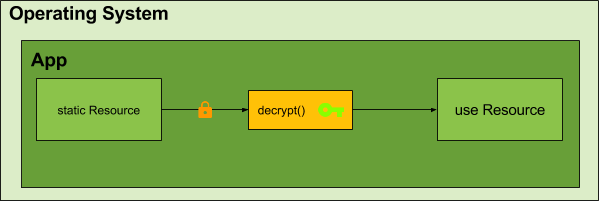
\includegraphics[width=0.8\textwidth]{data/encryptionResource.png}
    \caption{Encrypted resources have to be decrypted before they are used or displayed}
    \label{fig:encryptionResource}
\end{figure}

\subsubsection{Encryption - Action Obfuscator} \label{subsubsectionection:counter-replace-encryption-content-obfuscator}
The second approach is to use encryption as obfuscation.
The idea is to have a single method to deligate all other method calls according to an encrypted parameter.
\newline
When an attacker does a static analysis of the code, the links between method call and executing method are not apparent.
It forces the attacker to use a dynamic analysis method instead.
The fortification of the mechanism is improved when encrypted arguments are passed as well and the decryption is done in the executing method.
This requires more than just opcodes to be circumvented.
\newline
An abstract presentation of the mechanism can be seen in figure~\ref{fig:encryptionAction}.
\begin{figure}[h]
    \centering
    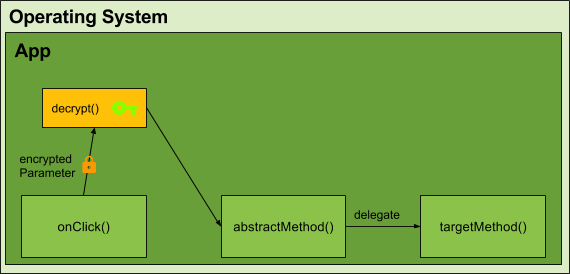
\includegraphics[width=0.8\textwidth]{data/encryptionAction.png}
    \caption{Encrypted actions to obfuscate dependencies}
    \label{fig:encryptionAction}
\end{figure}

\subsubsection{Communication} \label{section:counter-replace-encryption-content-communication}
The third approach is to use encryption on the server response as seen in figure~\ref{fig:encryptionComm}.
This is an additional security feature which is applied in combination with a content server described in subsection~\ref{section:counter-replace-server}.
When the user does the login on the server, additional unique device specific paramters have be passed as well.
On the first login, the server generates a cryptographic key which is used for communication with the user on this specific device.
The corresponding key can either be generated on the device or be shared by the server.
This mechanism allows only authorized users on a specific device to decrypt the communication.
\newline
\begin{figure}[h]
    \centering
    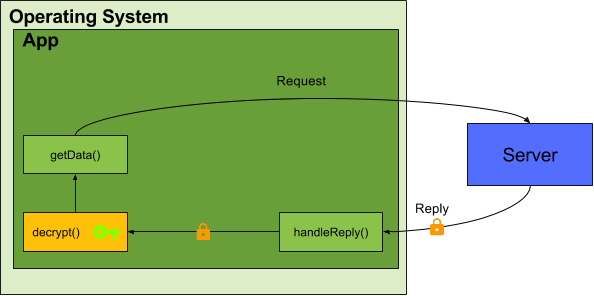
\includegraphics[width=0.8\textwidth]{data/encryptionComm.png}
    \caption{Encrypted communication with a server}
    \label{fig:encryptionComm}
\end{figure}

A similar approach is used for streaming \gls{drm} protected content on Android.
The encrypted content can only be decrypted by a native interface provided by the \gls{os} which stores the decryption key. \cite{androidDrm}
\newline
This methodology focuses on the security of the content instead of the application itself.

After applying encrpytion on the application, the handling of the key has to be specified.

\subsubsection{Key Storage - Online and Caching} \label{section:counter-replace-encryption-key-online}
The first approach to handle the encryption key is to store it on a server and provide it to the application.
This works similar to the license verification.
\newline
On decrypt method call, the application tries to retrieve a cached cryptographic key.
In case a cached key is available, the application starts to decrypt the content.
Otherwise the key is requested from the server.
The server does a verification of the user similar to the license verification libraries.
In case the check is successful, the decryption key is send to the device instead of a simple yes or no.
The advantage over having the original implementation is that the key can neither be accessed without the verification on the server and nor guessed by an attacker to circumvent this countermeasure.
\newline
The key can either be retrieved from the server for each decryption action or it can be cached on the device, similar to the license verification policy.
Caching should be favored since getting the key for each action not only requires to be online but slows down the application and generates additional traffic.
\newline
In order to improve security, keys can be changed when updating the version of the application or be user specific.
\begin{figure}[h]
    \centering
    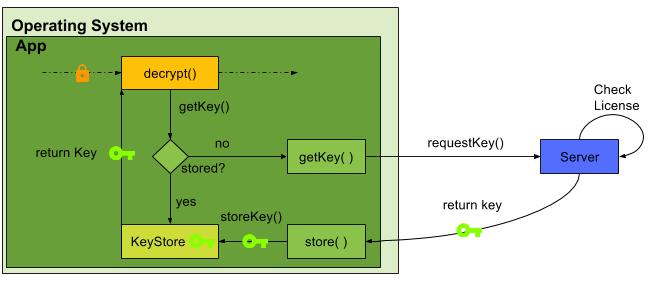
\includegraphics[width=0.8\textwidth]{data/encryptionKeyServer.png}
    \caption{Retrieving the key after successful identification from the server and store it local on device}
    \label{fig:encryptionKeyServer}
\end{figure}

\subsubsection{Key - Secure Element} \label{section:counter-replace-encryption-key-local}
Since there is the possibility to read the cached encryption key \cite{memoryDump} and crack the encryption, the use of \gls{se} is proposed.
A secure element is a tamper-resistant platform which can be used to securely host applications and cryptographic keys \cite{seDefinition}.
There are different form factors for \gls{se}s.
For Android, the microSD form factor is the interesting one.
It can be either mounted in the microSD card slot or by using an adapter on the USB interface, which requires the device to support \gls{otg} \cite{usbOtg}.
The resource is accessed over reads and writes to the filesystem.
Since the \gls{se} has to be small to fit the size of an microSD card and powered by the host system, its hardware capabilities are constrained.
The result is a performance of 25MHz which does not allow complexe comnputations. \cite{stSe}
\newline
For this reason the usage of the \gls{se} is restricted to simple tasks, like storing a key used for decryption.
The advantage of an \gls{se} is that its functionality is outside of the Android application and thus cannot be manipulated by \gls{luckypatcherg}.
\newline
An abstract presentation of the use of a \gls{se} can be seen in figure~\ref{fig:encryptionKeySmart}.
\newline
\begin{figure}[h]
    \centering
    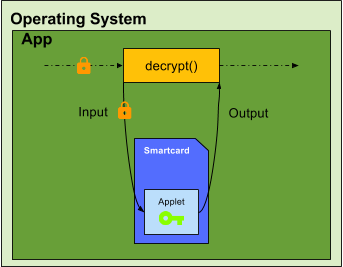
\includegraphics[width=0.8\textwidth]{data/encryptionKeySmart.png}
    \caption{Decryption by using a smartcard}
    \label{fig:encryptionKeySmart}
\end{figure}
Integrating a \gls{se} comes with some problems.
\begin{itemize}
  \item the user has to buy extra hardware
  \item not all devices have a microSD card slot or support \gls{otg}
  \item different implementations for communication with the \gls{se}
\end{itemize}
The first problem is that the user is required to buy extra hardware.
This means the user has to spend extra cache and to have the \gls{se} always around.
The connection to the device using a cable is not the most convenient solution as well.
The second problem is that not all devices either have an microSD card slot, nor \gls{otg} support.
For example, the Nexus 7 (2012) and the Nexus 6P neither have the capability to use a microSD card.
While the Nexus7 was supposed to have \gls{otg}, it did not work with the used \gls{se}, while the Nexus 6P did not support \gls{otg} out of the box.
Both devices needed even needed additional plugins to read the \gls{otg} mounted microSD in a file explorer.
The third problem is that each manufacturer implements its own interpretation for the interface which makes \gls{se} incompatible to each other.
For this reason, the SD Association proposed the smartSD in order to have a universal standard for \gls{se}s \cite{smartSD}.
\newline


se signiert mit key+android\_id welche unique ist

TODO:
2) Secure Elements
Bottleneck ist sicherlich die Schnittstelle zu Android und alles was in Android ist, ist prinzipiell unsicher, also auch etwaige Keys. Was jedoch koennte Secure Elements absichern? Ich moechte dich bitten hier Ideen zu erarbeiten, was im Zuge von Kopierschutz,  Verschluesslung etc. mit SEs wirklich sicher gemacht werden koennte. Eine grobe Idee ist z.B. das Signieren von Serveranfragen. Key kennt hier nur das SE und der Server. Android schickt die volle URL mit Parametern und das SE fuegt einen Signaturparameter zu. Vorteil: Ohne das SE kann die App den Server mal nicht mehr nutzen. Jetzt musste man verhindern, dass eine Proxy-App unter Android fuer andere aktiv wird (Stichwort CardSharing). Was koennte man tun? Das ist auch nur ein Idee. Was gibt es sonst noch? Wo koennte es Sinn machen einen sicheren Speicher zu haben?

